\begin{comment}
\begin{itemize}
  \item Glomal350(https://www.aisan.co.jp/products/glomal350.html)
  \item WORLDEYE(https://www.gakkensf.co.jp/worldeye/sp/)
  \item OmniEyeball: An Interactive I/O Device For 360-Degree Video Communication(https://dl.acm.org/doi/10.1145/3279778.3279926)
  \item Qoom: An Interactive Omnidirectional Ball Display(https://dl.acm.org/doi/10.1145/3126594.3126607)
  \item Comparing flat and spherical displays in a trust scenario in avatar-mediated interaction(https://dl.acm.org/doi/10.1145/2556288.2557276)
\end{itemize}
\end{comment}

\subsubsection*{球体ディスプレイ}

球体ディスプレイの例として,渋谷工学のGlomal350\cite{15}や学研の
WORLDEYE\cite{22},WataruらのiSphere\cite{23}がある.
球体ディスプレイには
\begin{itemize}
  \item リアプロジェクション型
  \item フロントプロジェクション型
  \item 発光型
\end{itemize}

の3種類が存在する.リアプロジェクション型は,ディスプレイの裏側から
映像投影を行う.フロントプロジェクション型は,ディスプレイの外側から
映像投影を行う.一方で,発光型は,球の構成自体を,有機EL等の
発光装置で行い,球それ自体が発光する.Glomal550やWORLDEYEは,リアプロジェクション型
の球体ディスプレイである.
一方でiSphereは,ドローンに発光LEDを取り付けて回転させて球状
映像を表示する,発光型の球体ディスプレイである.(表\ref{isphere})
\begin{figure}[tbp]
  \centering
  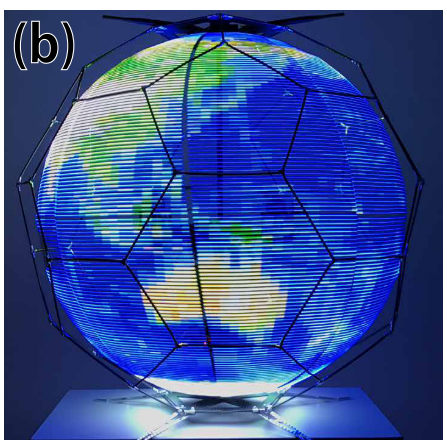
\includegraphics[scale=1.0]{fig/isphere.png}
  \caption{iSphere\cite{23}}\label{isphere}
\end{figure}

リアプロジェクション型の球体ディスプレイは,球内部に
魚眼レンズを取り付けており,また殆どの魚眼レンズは
等距離射影方式を採用している.等距離射影方式は,
レンズへの光の入射角を$\theta$,スクリーンへの
光の到達点と光軸との距離を$R$,焦点距離を$f$とすると
以下の式が成り立つ射影方式である.(図\ref{pro})

\begin{eqnarray}
  R = f\theta \nonumber \\
\end{eqnarray}

\begin{figure}[tbp]
  \centering
  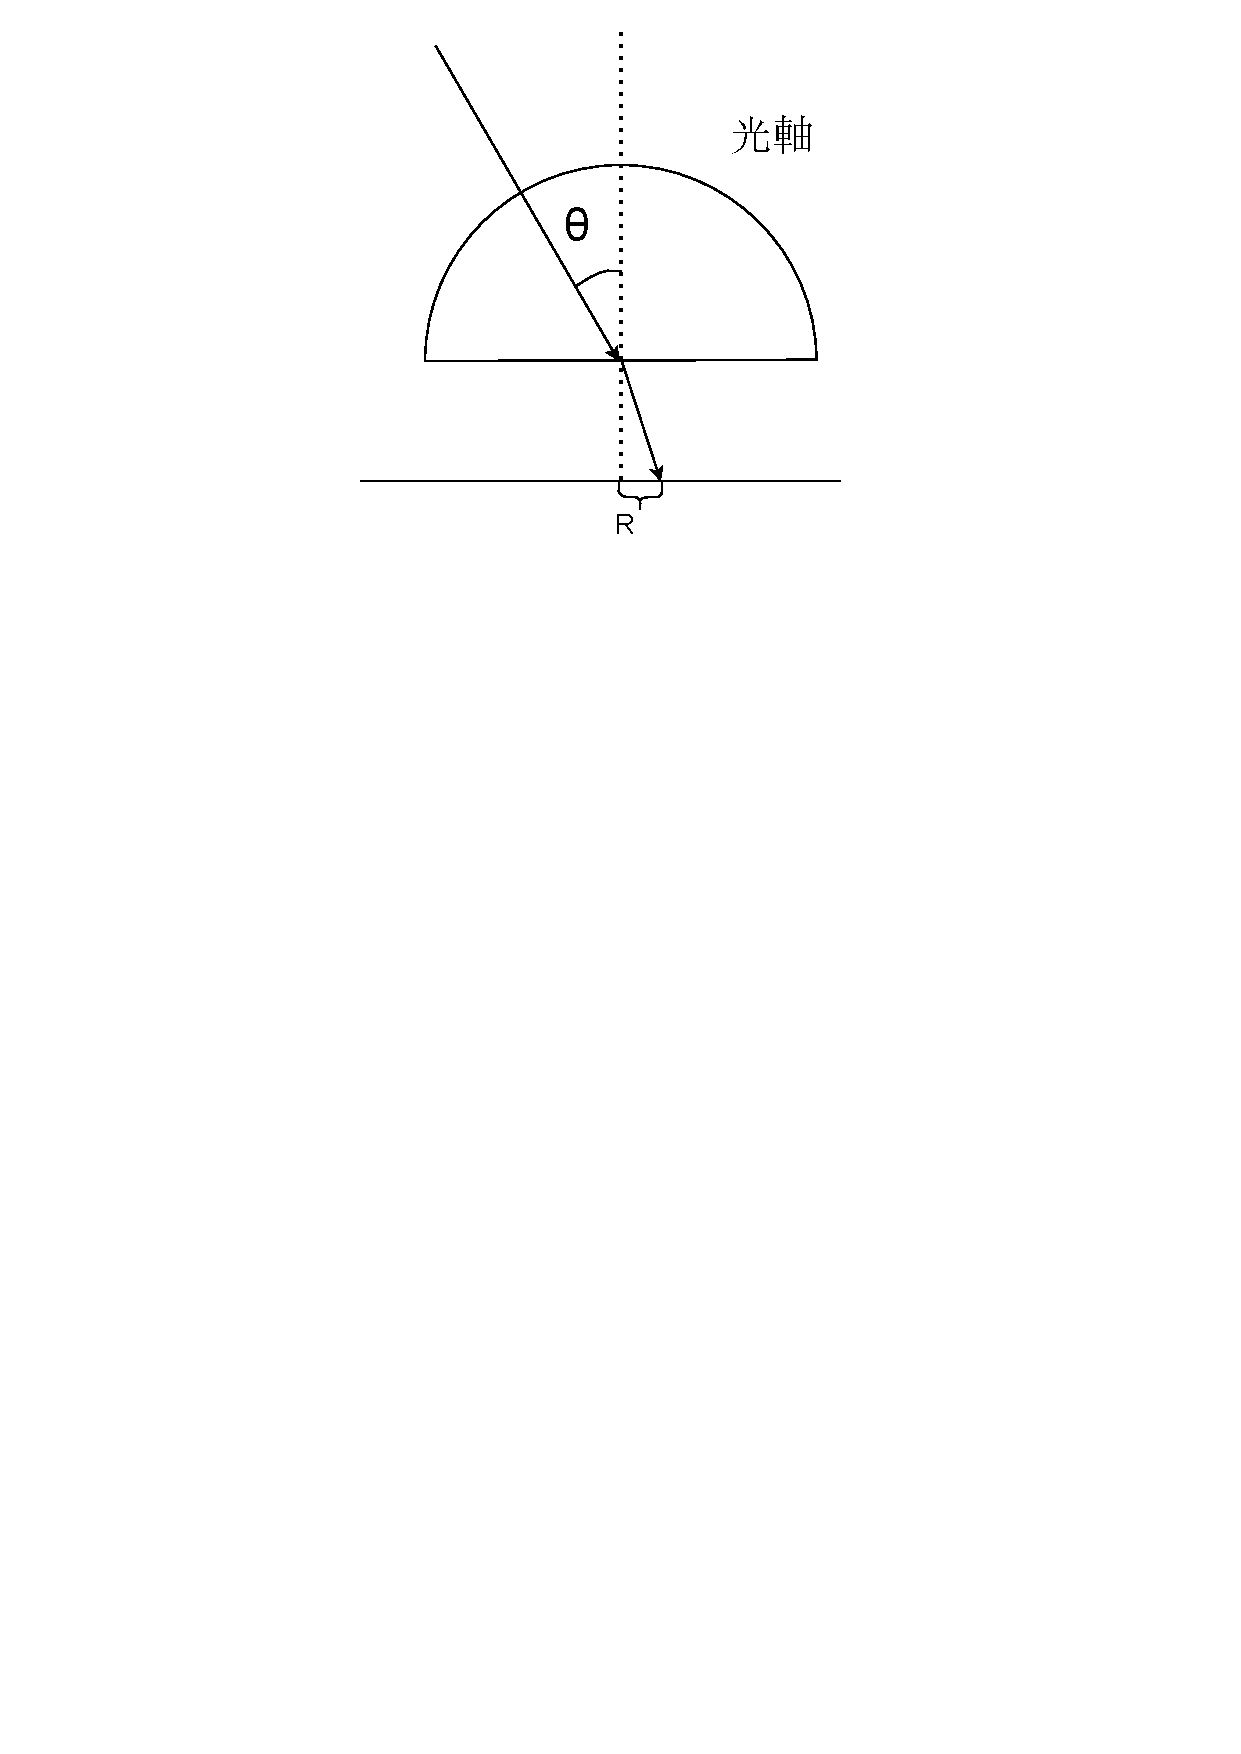
\includegraphics[scale=0.7]{fig/projection2.pdf}
  \caption{等距離射影方式の模式図}\label{pro}
\end{figure}

すなわち,投影元の画像中心からの距離に比例して,投影先の球体上での
天頂からの角度が比例する.よって,魚眼レンズを使用したリアプロジェクション型の
球体ディスプレイを利用する際には,投影元の映像を正距方位図法(図\ref{teiso3})へと
変換しておく必要がある.

\begin{figure}[tbp]
  \centering
  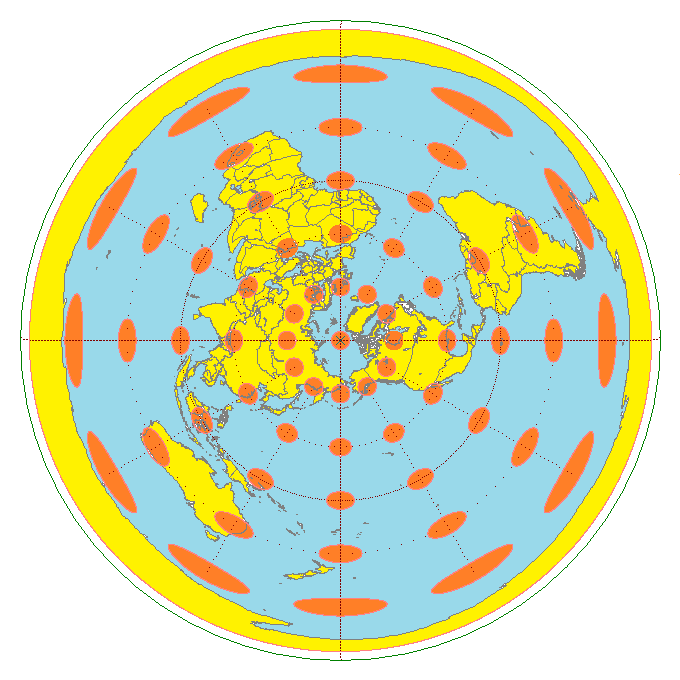
\includegraphics[scale=0.8]{fig/teiso3.png}
  \caption{正距方位図法\cite{20}}\label{teiso3}
\end{figure}

\subsubsection*{球体ディスプレイの応用}
球体ディスプレイと全天球ビデオカメラを用いた例として,Liらの
OmniEyeBall\cite{18}\cite{24}がある.OmniEyeBallは,
glomal350を映像プロジェクターとして用いて,球体ディスプレイの
天頂部に広角の魚眼レンズを取り付けたデバイスである.(図\ref{proto})
\begin{figure}[tp]
  \centering
  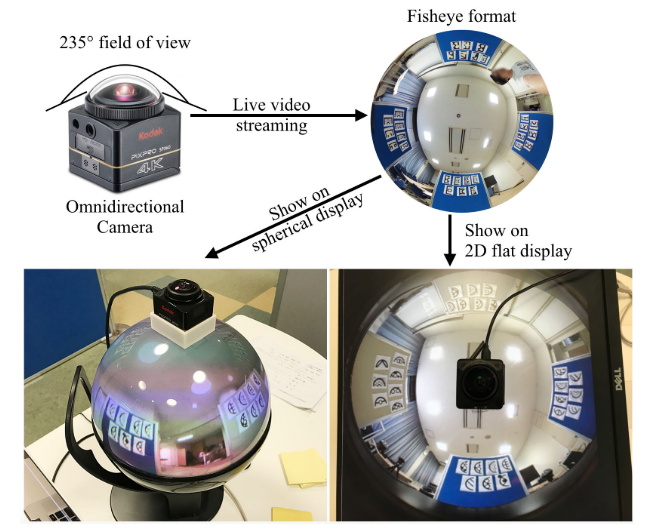
\includegraphics[scale=0.6]{fig/OEBproto.png}
  \caption{OmniEyeBallの構成の概要\cite{24}}\label{proto}
\end{figure}

2台のOmniEyeBallを用いて,魚眼レンズの映像のストリーミングを行うことで,
OmniEyeBallを複数人で囲う形のビデオ会議が可能である.
OmniEyeBallをもちいたビデオ会議実験では,平面ディスプレイでの表示では
歪みが強い,球体ディスプレイでの表示は距離や方向感覚がつかみやすい
といった内容が報告されている.また球体ディスプレイを用いた方が
特定の個人とのコミュニケーションがしやすくなったことが示されており,
一方で平面ディスプレイ時には多対多のコミュニケーションが多く行われたことが
示された.

Miyafujiら\cite{25}は,複数のプロジェクターとモーションキャプチャーを
利用して,動くボールに対してプロジェクションマッピングを行い,ボールを
フロントプロジェクション型の球体ディスプレイとして利用するQoomを提案した.
Qoomでは,ボールに対して触れる,回す,地面に投げる,人に投げるといった,人が
ボールに対して行う自然な動作に対して,それぞれに対応した挙動をするように設計されている.

\begin{figure}[tbp]
  \centering
  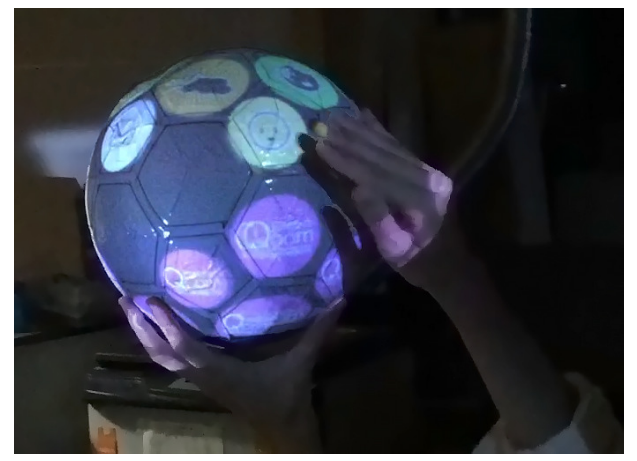
\includegraphics[scale=0.9]{fig/qoom.png}
  \caption{Qoom\cite{25}}
\end{figure}

\begin{figure}[tbp]
  \centering
  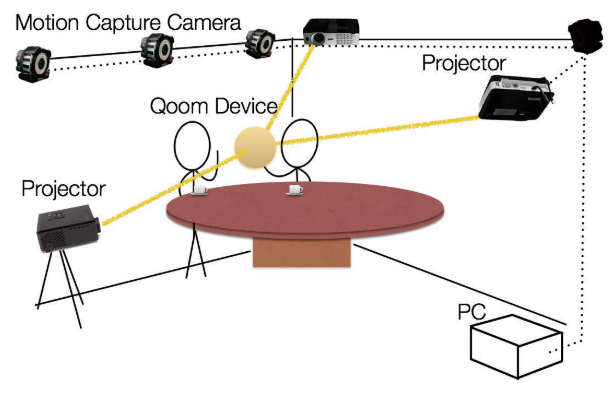
\includegraphics[scale=1.0]{fig/qoomsys.png}
  \caption{Qoomの構成の概要\cite{25}}
\end{figure}

Panら\cite{26}は,平面ディスプレイと球体ディスプレイで
アバターの表示に関する比較の研究を行った.実験の内容は,
30個の難解な質問に対し,声と容姿は同一で正答率の異なるアバターを,
平面ディスプレイと球体ディスプレイのそれぞれに表示し,どちらか片方のみから
答えを聞くというものであった.(図\ref{avaterexp})結果,被検者は球体ディスプレイの
アバターを多く選択する結果が得られている.特に,ディスプレイの距離
の差が広いほど,球体ディスプレイを選択する傾向にあったことが示された.
被検者のアンケートでは,アバターの動きや声の演者は同一であるのにもかかわらず
\begin{itemize}
  \item エマの目はサポート感があるが、ケイティの声の方が説得力がある
  \item ケイティはいつも答えに自信があるように見えるが、エマは自分の知っていることを話しているように見える
\end{itemize}
などの意見が見られていた.

\begin{figure}[tbp]
  \centering
  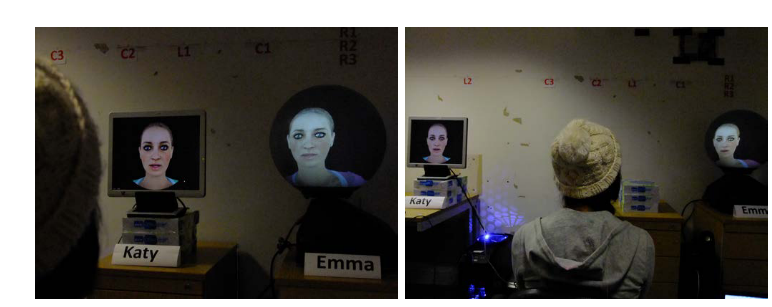
\includegraphics[scale=0.6]{fig/avaterexp.png}
  \caption{Panらの実験の様子\cite{26}}\label{avaterexp}
\end{figure}


